\chapterimage{Chapter20.jpg} % Chapter heading image

\chapter{Pumps and Pumping}


\section{Important conversions and formulas}\index{Important conversions and formulas}

Total dynamic head = Friction head + Static head\\
\vspace{0.3cm}
$1Hp=0.746kW$\\
\vspace{0.3cm}
$1Hp=\dfrac{33,000 \enspace ft-lb}{min}$\\
\vspace{0.3cm}
$1Hp=3,960 \enspace GPM-ft$\\
\vspace{0.3cm}
$1psi=2.31ft$\\
\vspace{0.3cm}
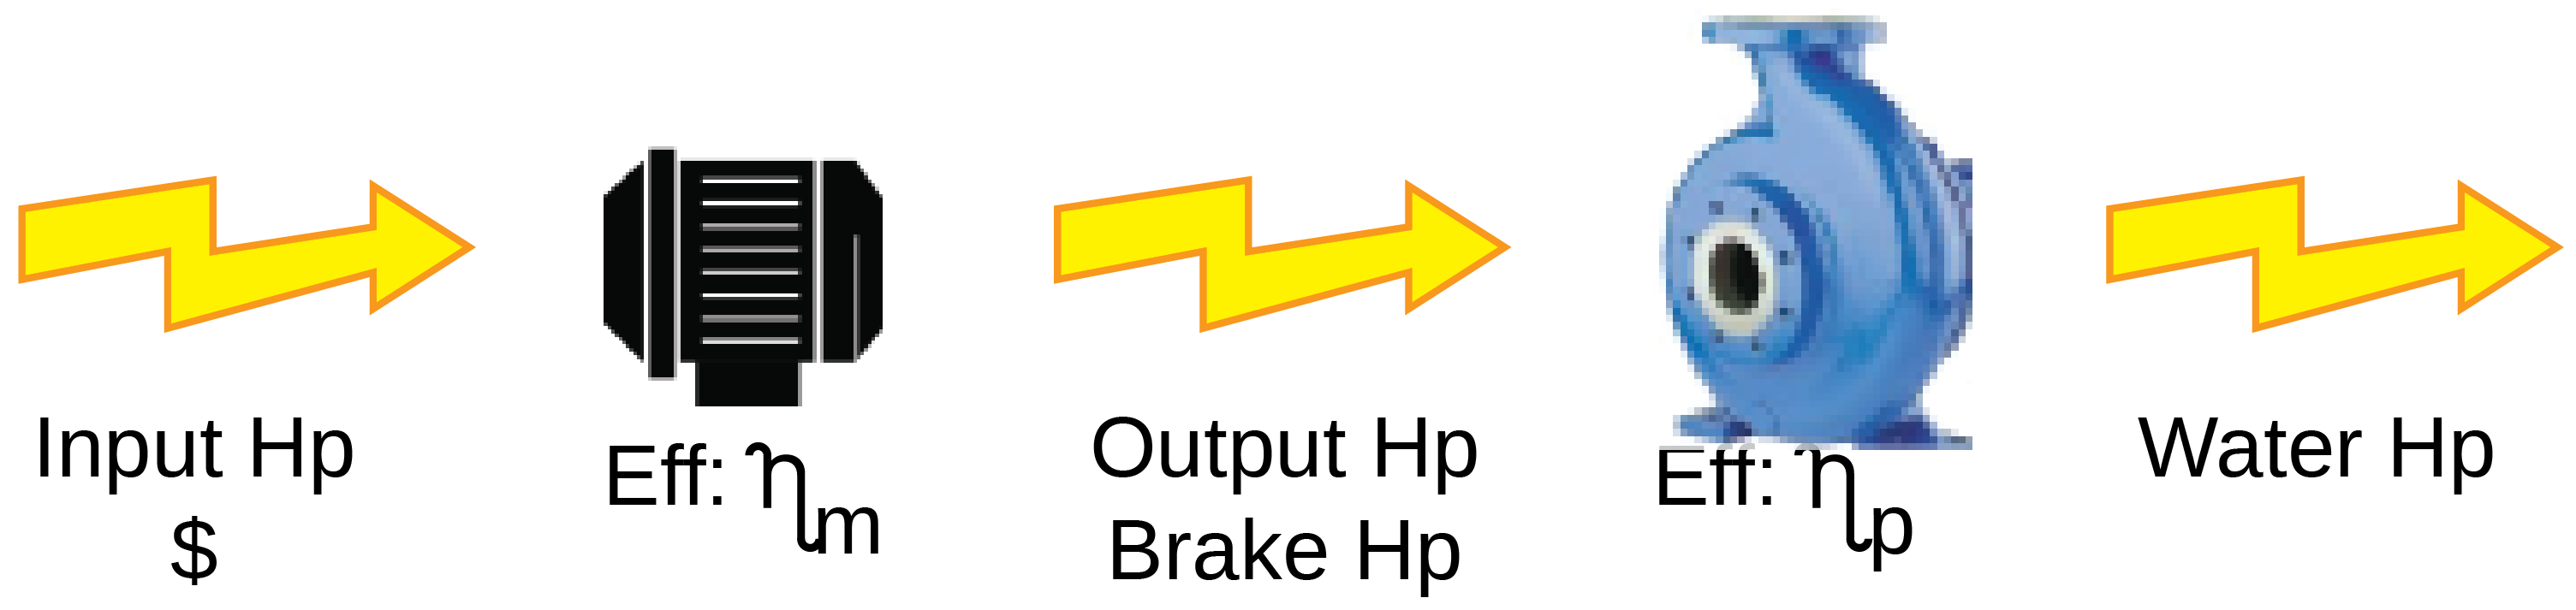
\includegraphics[scale=0.08]{PumpProblem}\\
\vspace{0.3cm}
$Water \enspace Hp \enspace = \enspace Flow \enspace *  \enspace Head$\\
\vspace{0.3cm}
$Brake  \enspace Hp \enspace = \enspace Input \enspace Hp*Motor \enspace efficiency$\\
\vspace{0.3cm}
$Water  \enspace Hp \enspace = \enspace Brake \enspace Hp \enspace * \enspace Pump  \enspace efficiency,  \enspace and$\\
\vspace{0.3cm}
$\implies Water  \enspace  Hp \enspace = \enspace Input  \enspace  Hp \enspace * \enspace Motor  \enspace efficiency \enspace * \enspace Pump  \enspace efficiency$\\

\newpage
\thispagestyle{empty}
% \begin{landscape}
% 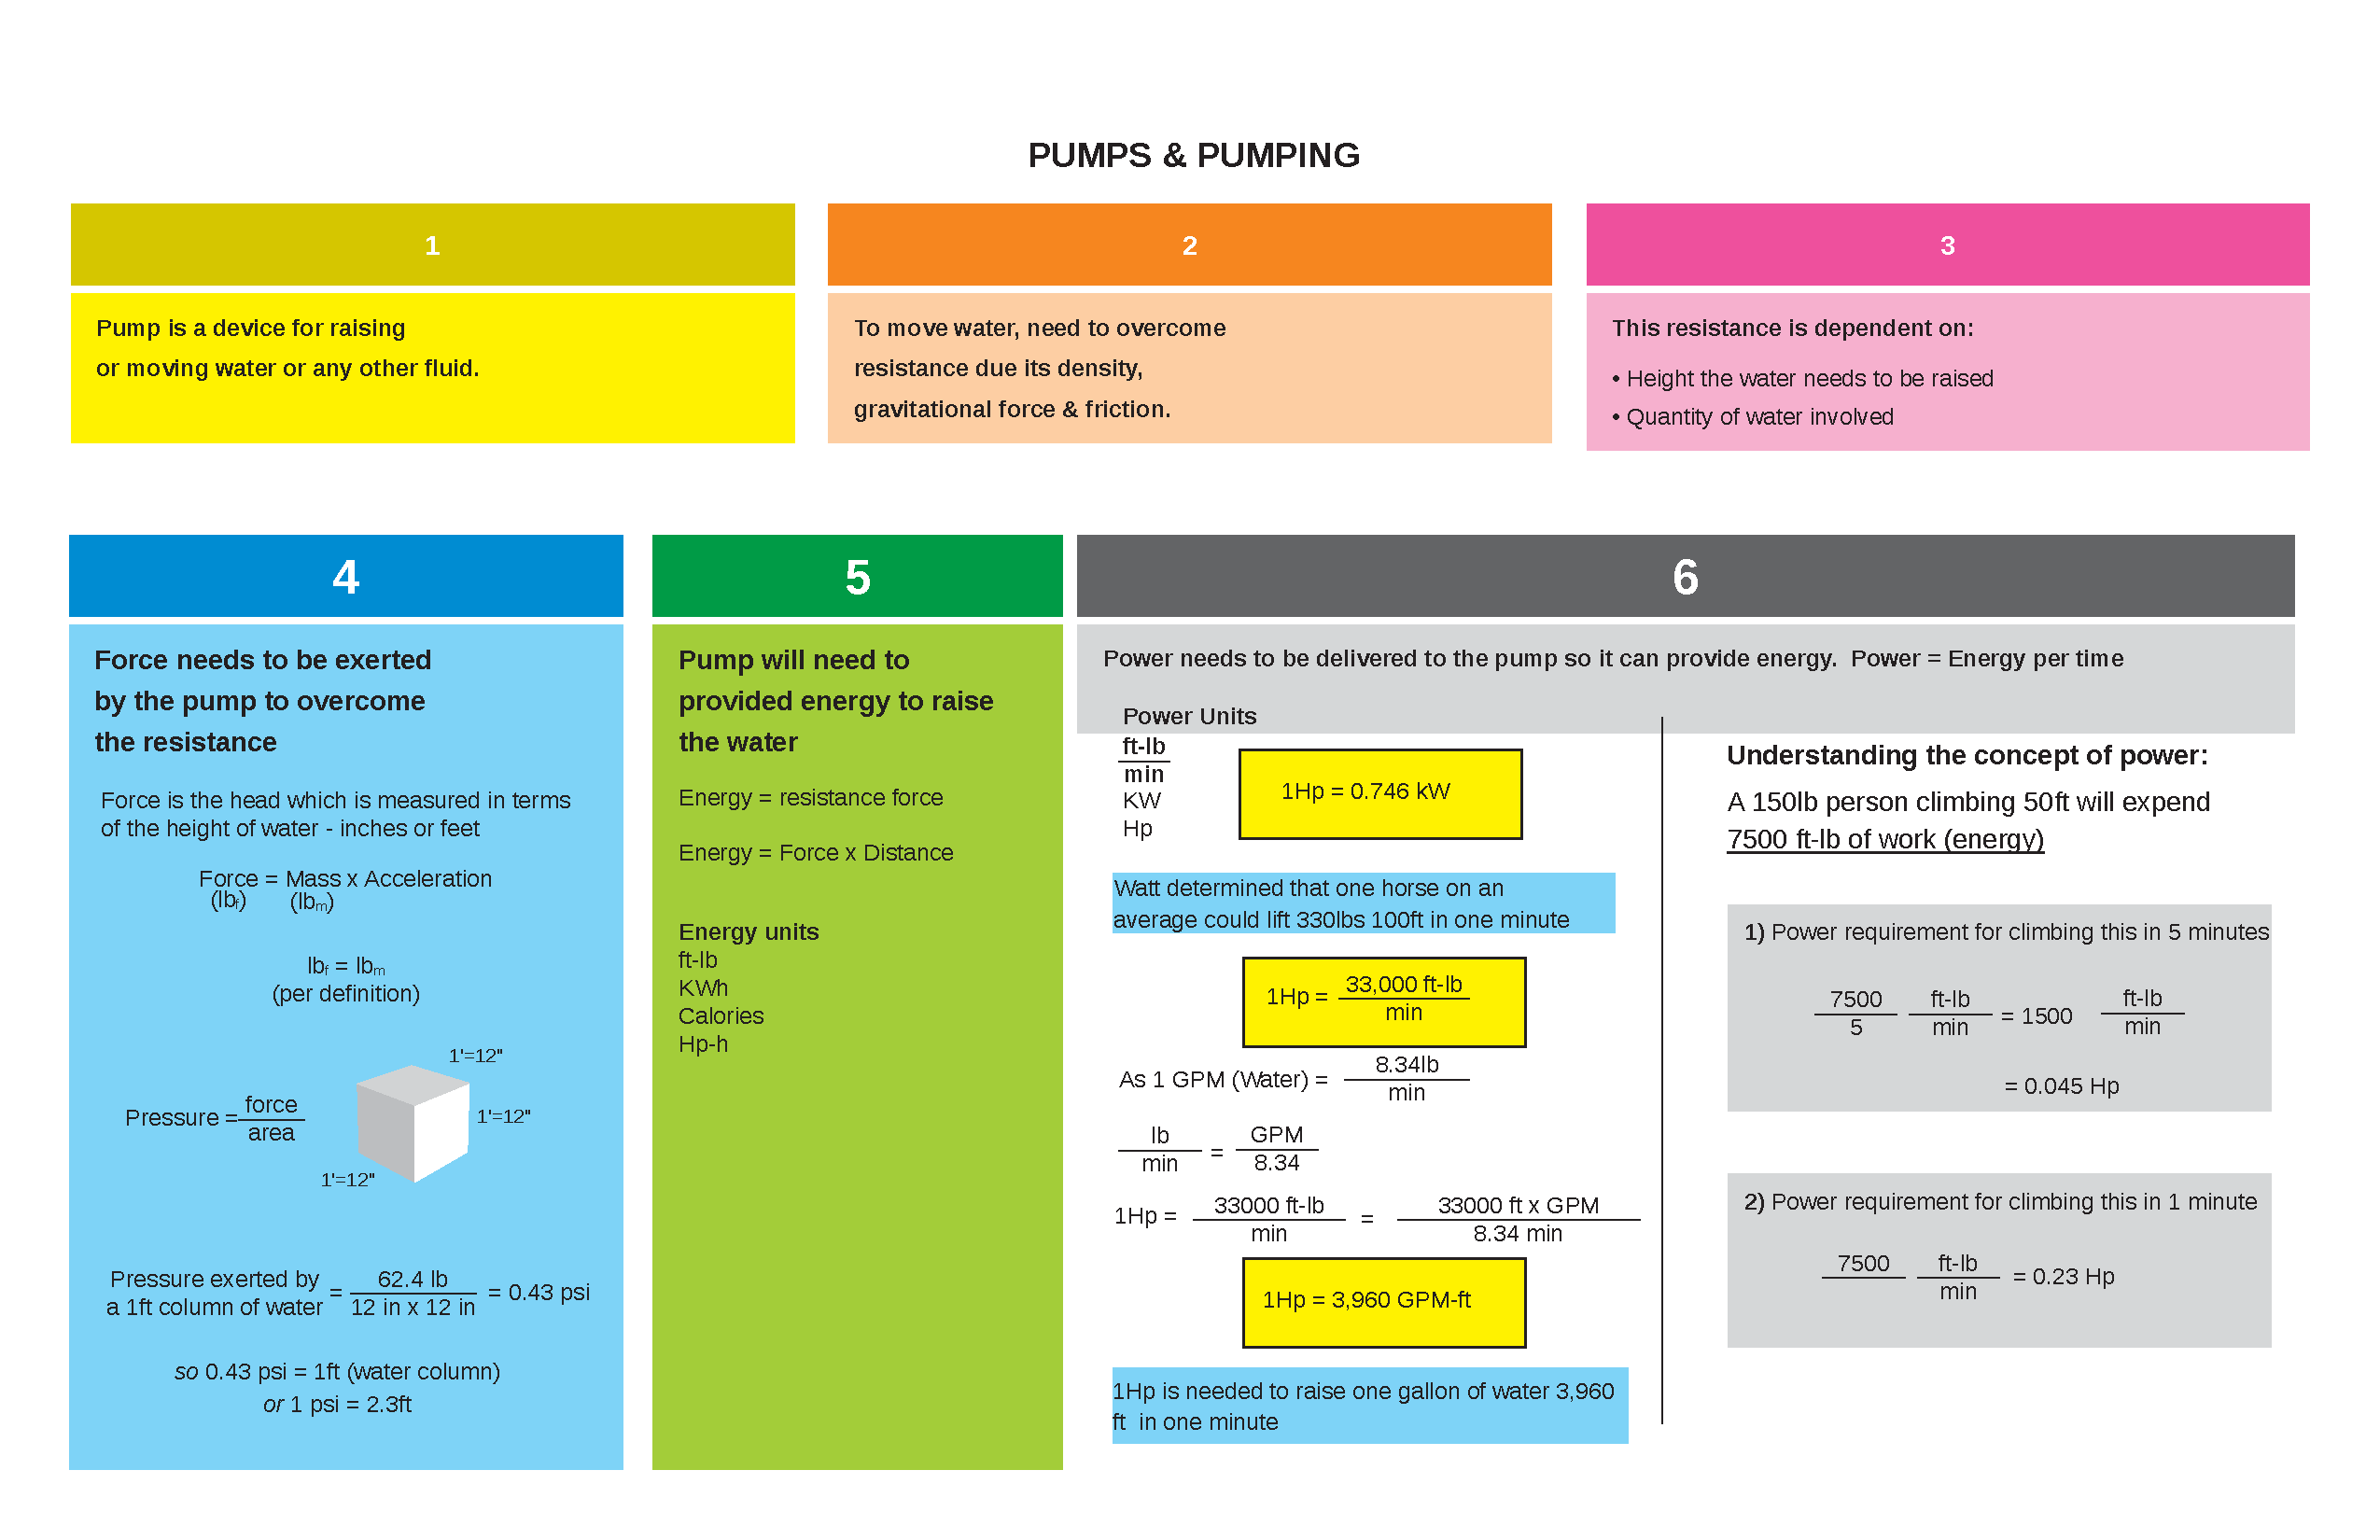
\includegraphics[scale=0.52]{PumpsandPumpingR1_01.pdf}
% \end{landscape}
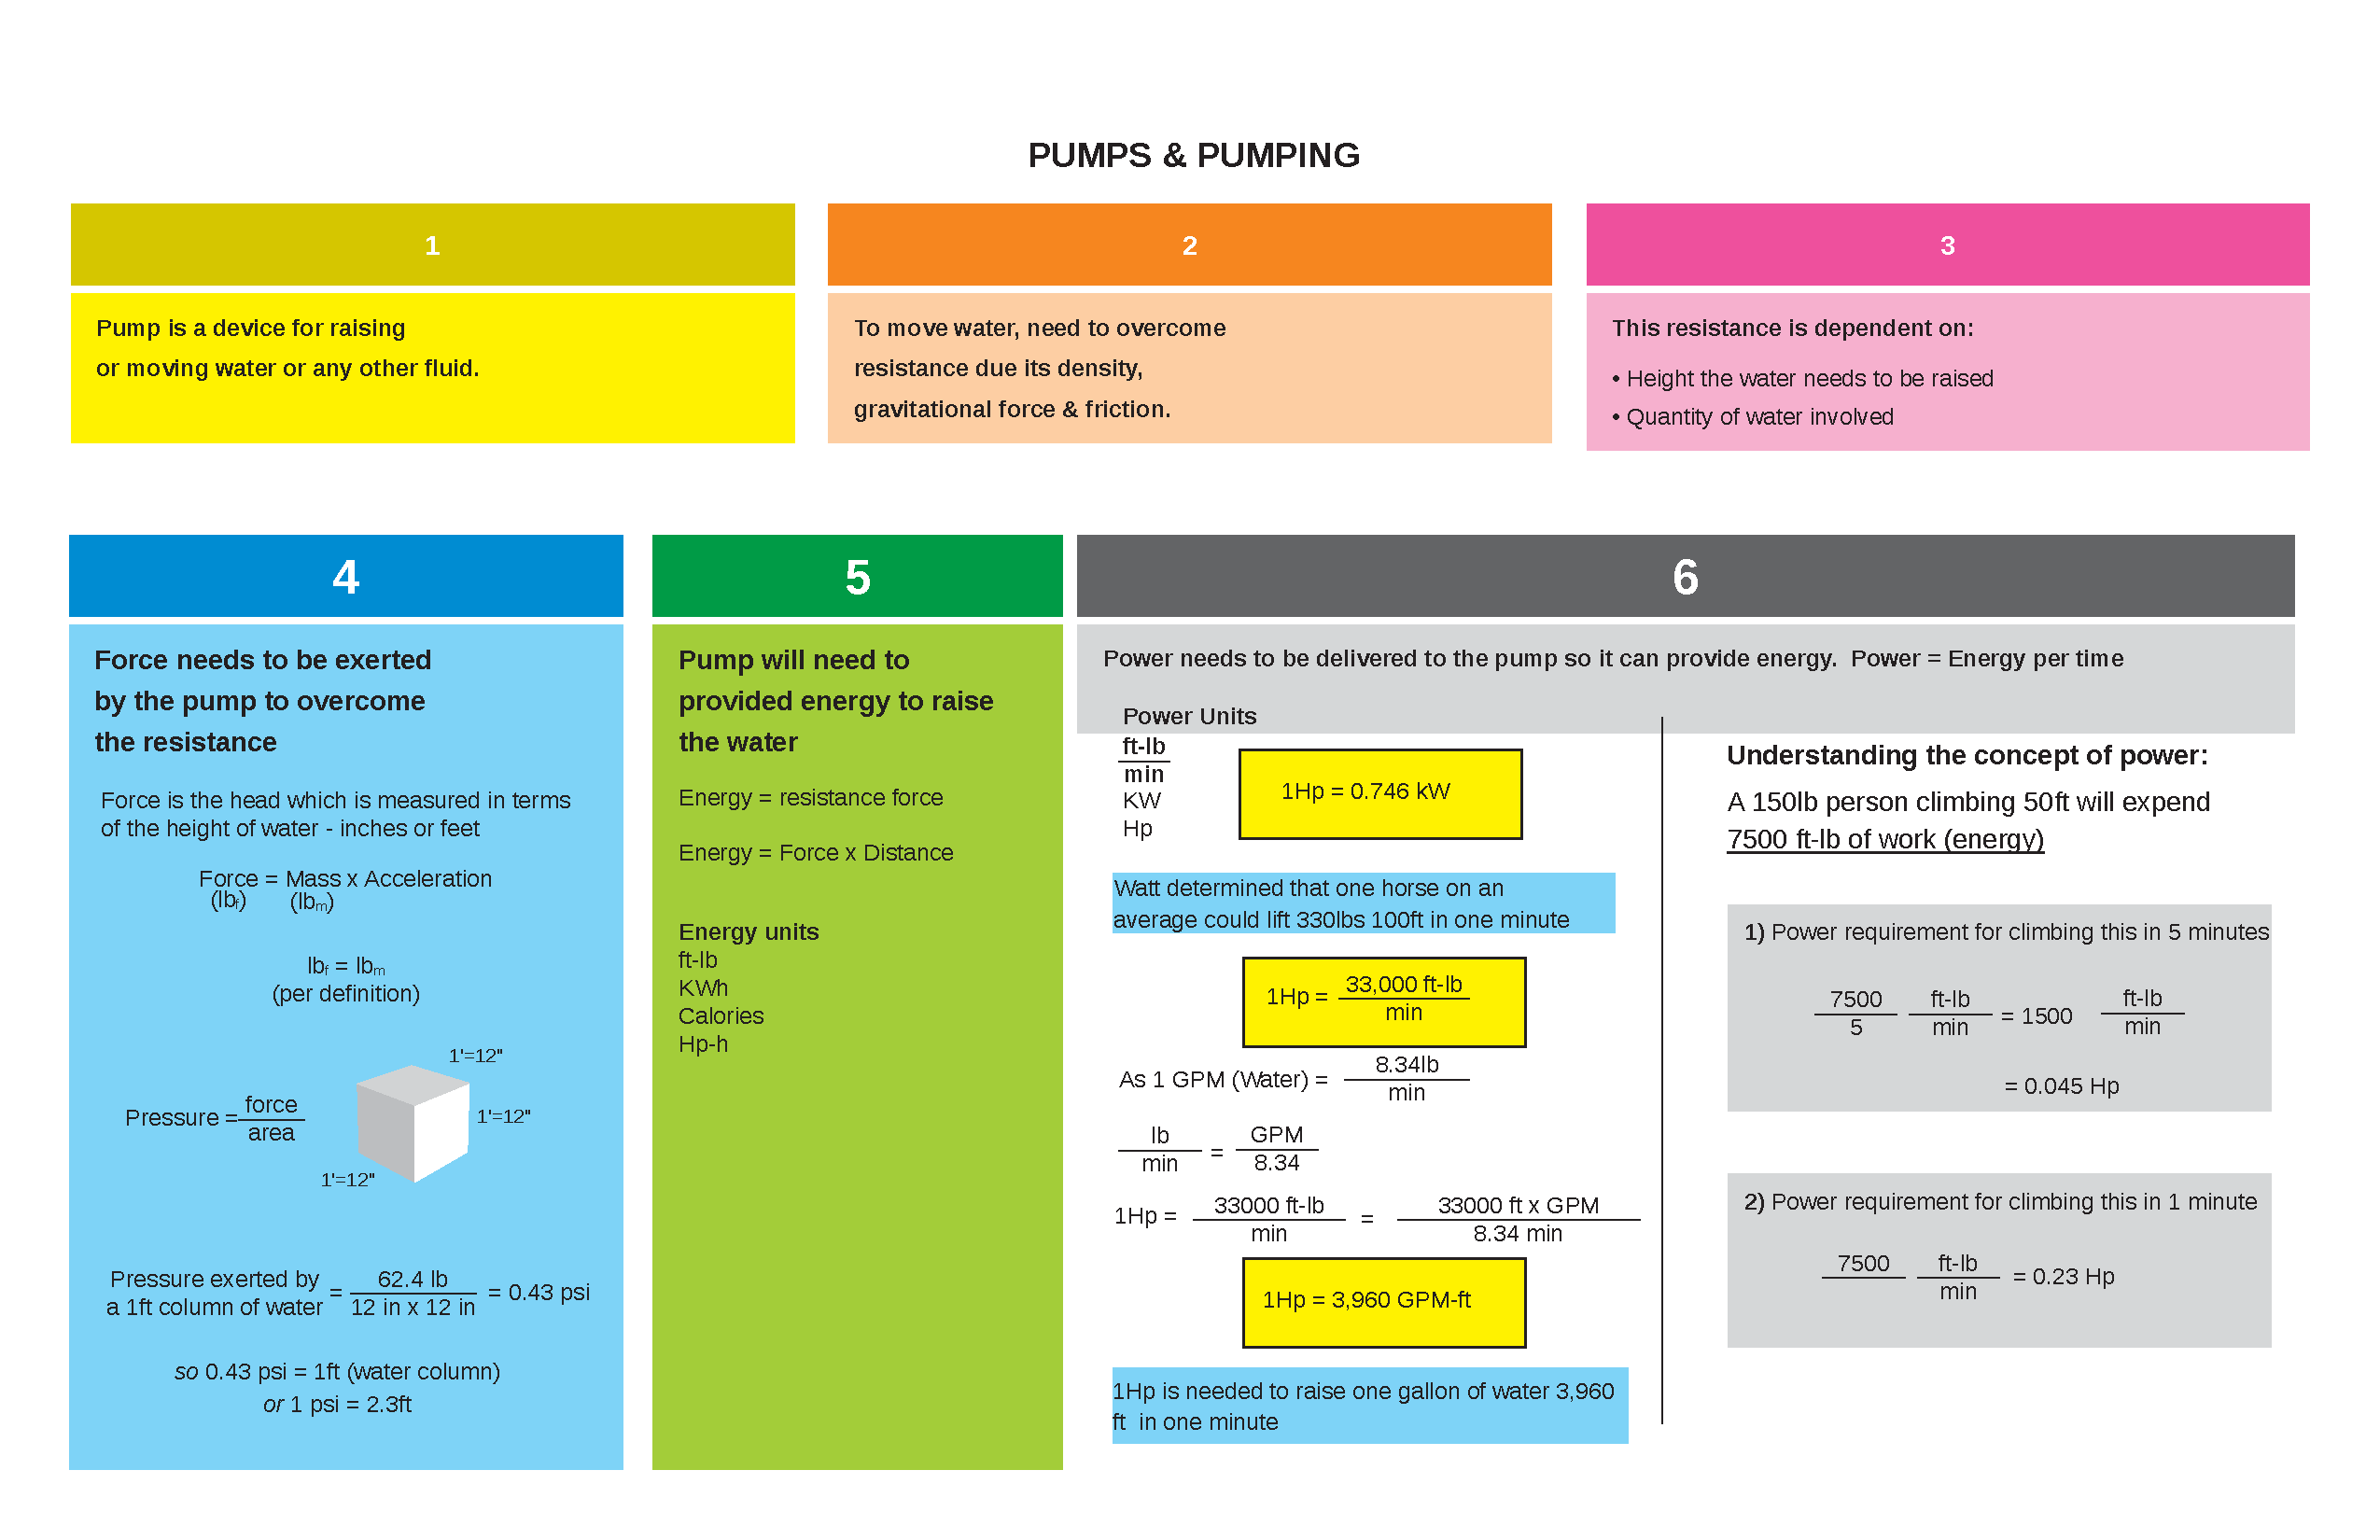
\includepdf[landscape=true]{PumpsandPumpingR1_01.pdf}
\newpage

\thispagestyle{empty}
% \begin{landscape}
% 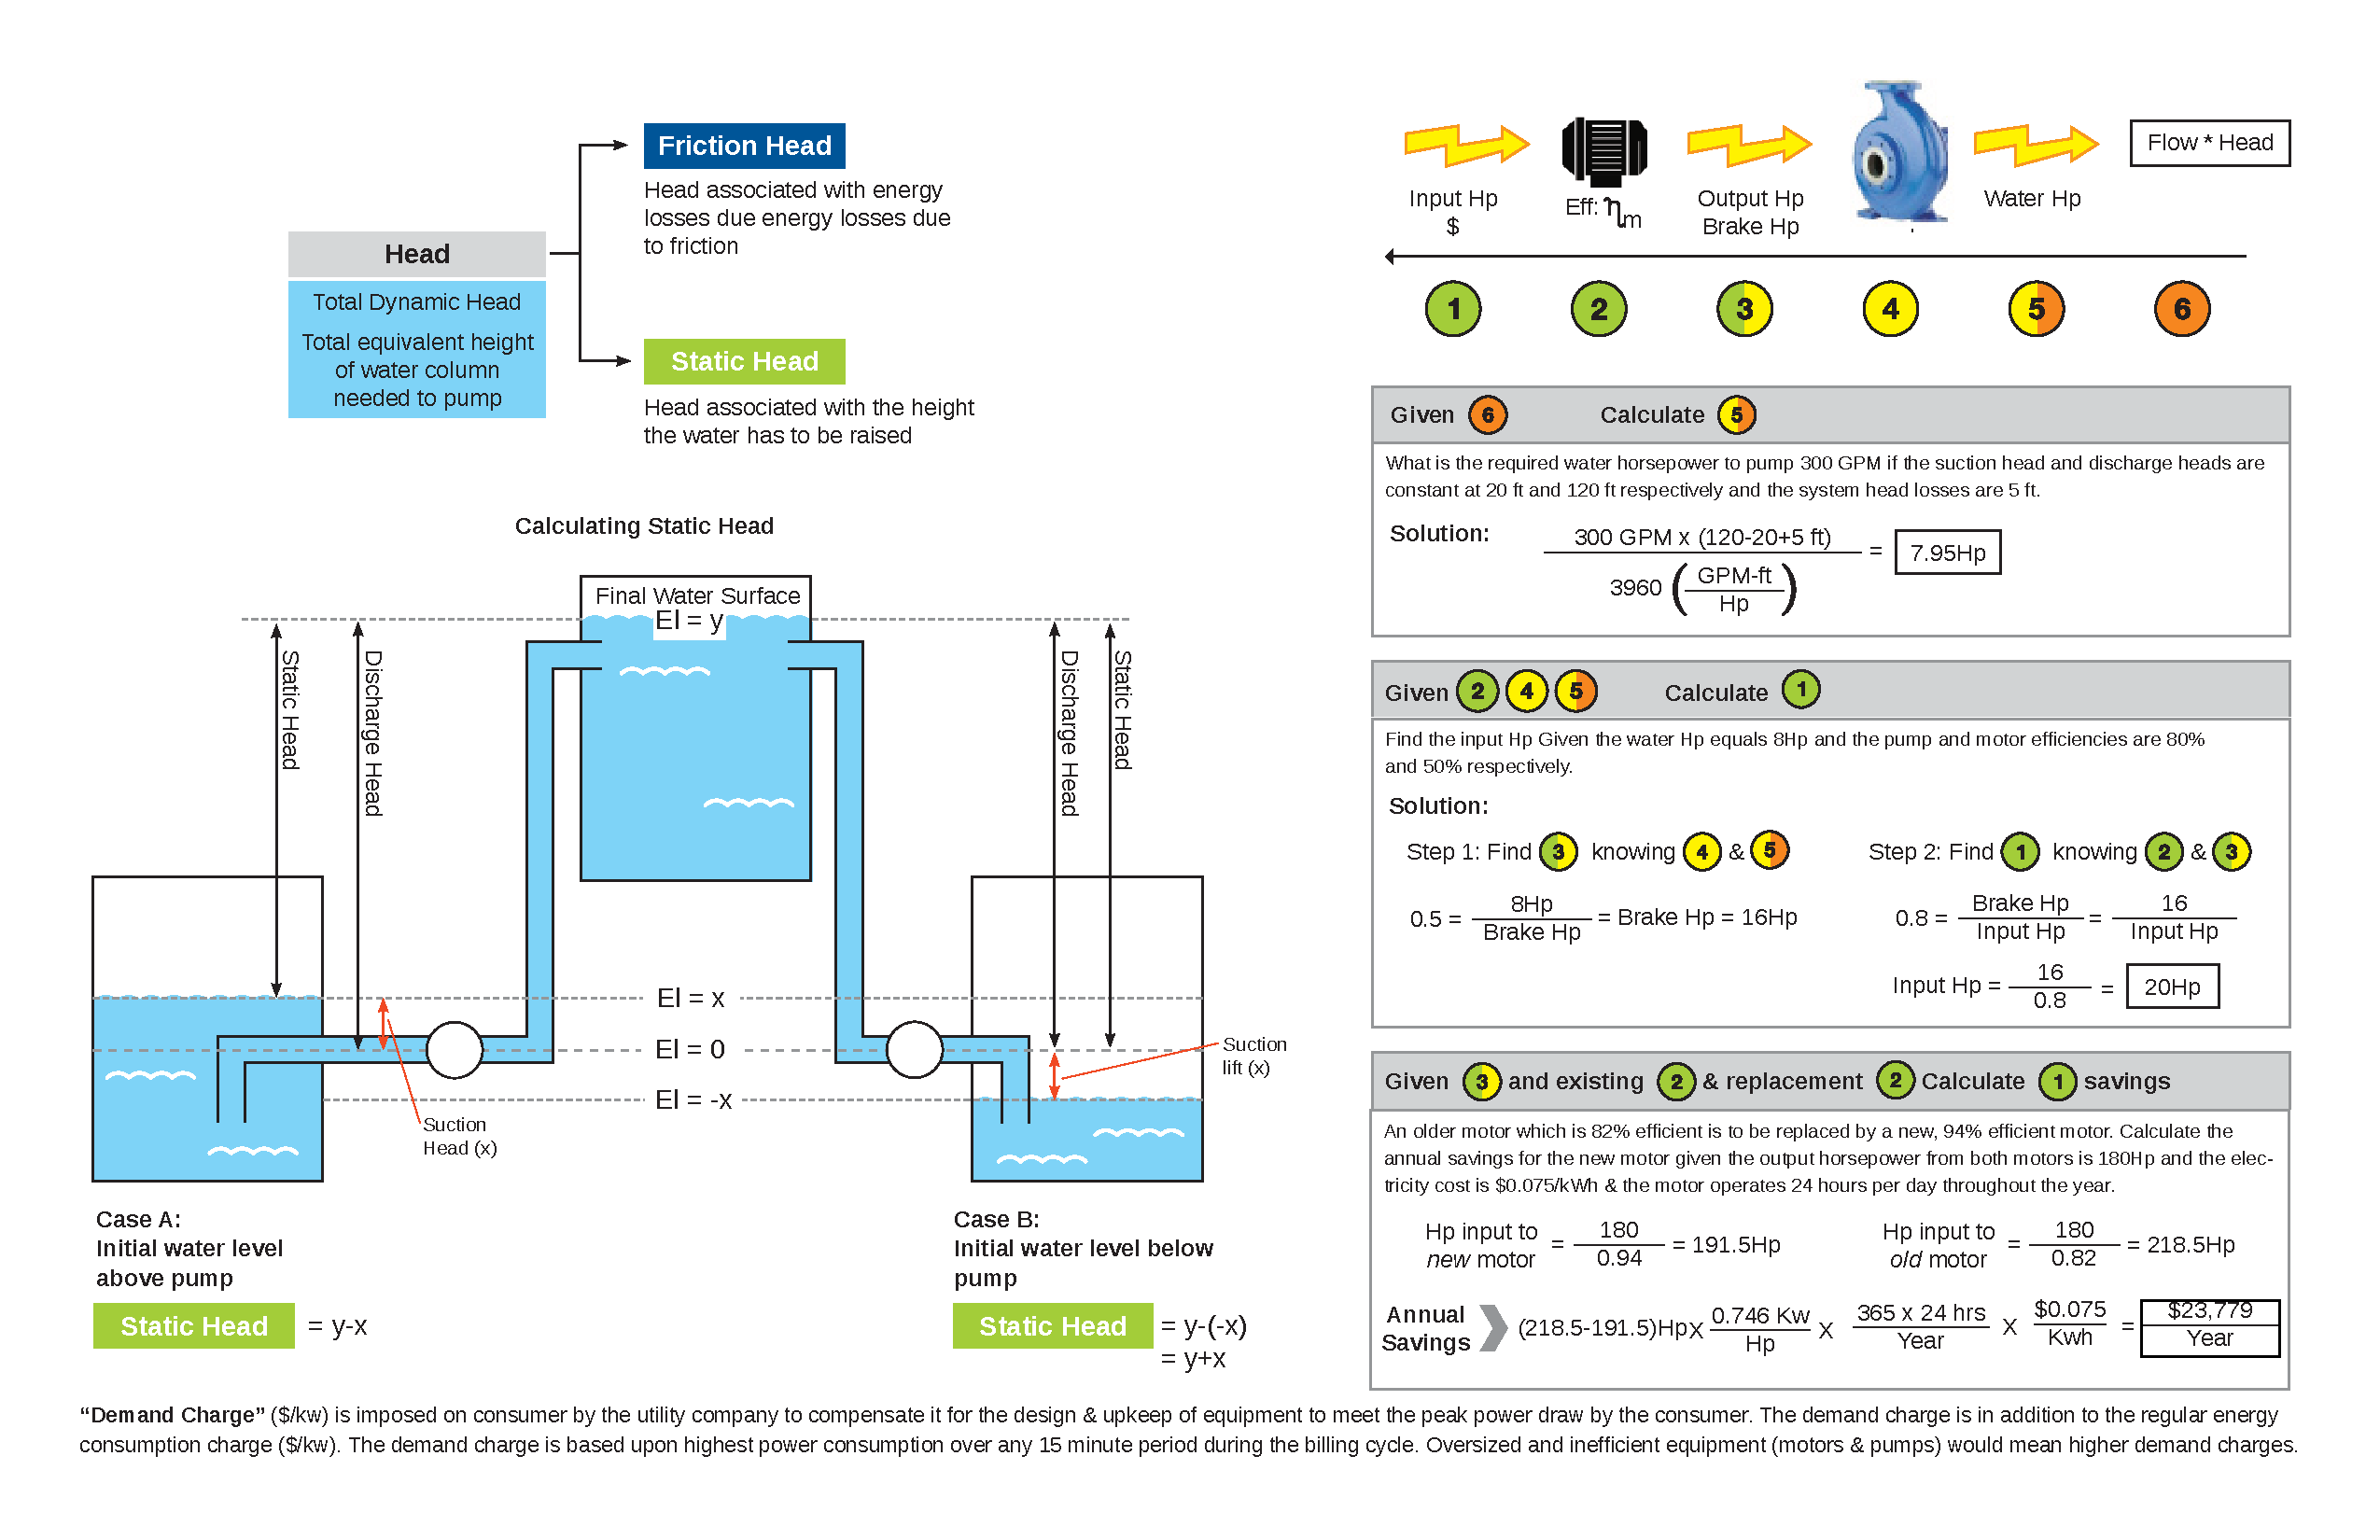
\includegraphics[scale=0.52]{PumpsandPumpingR1_02.pdf}
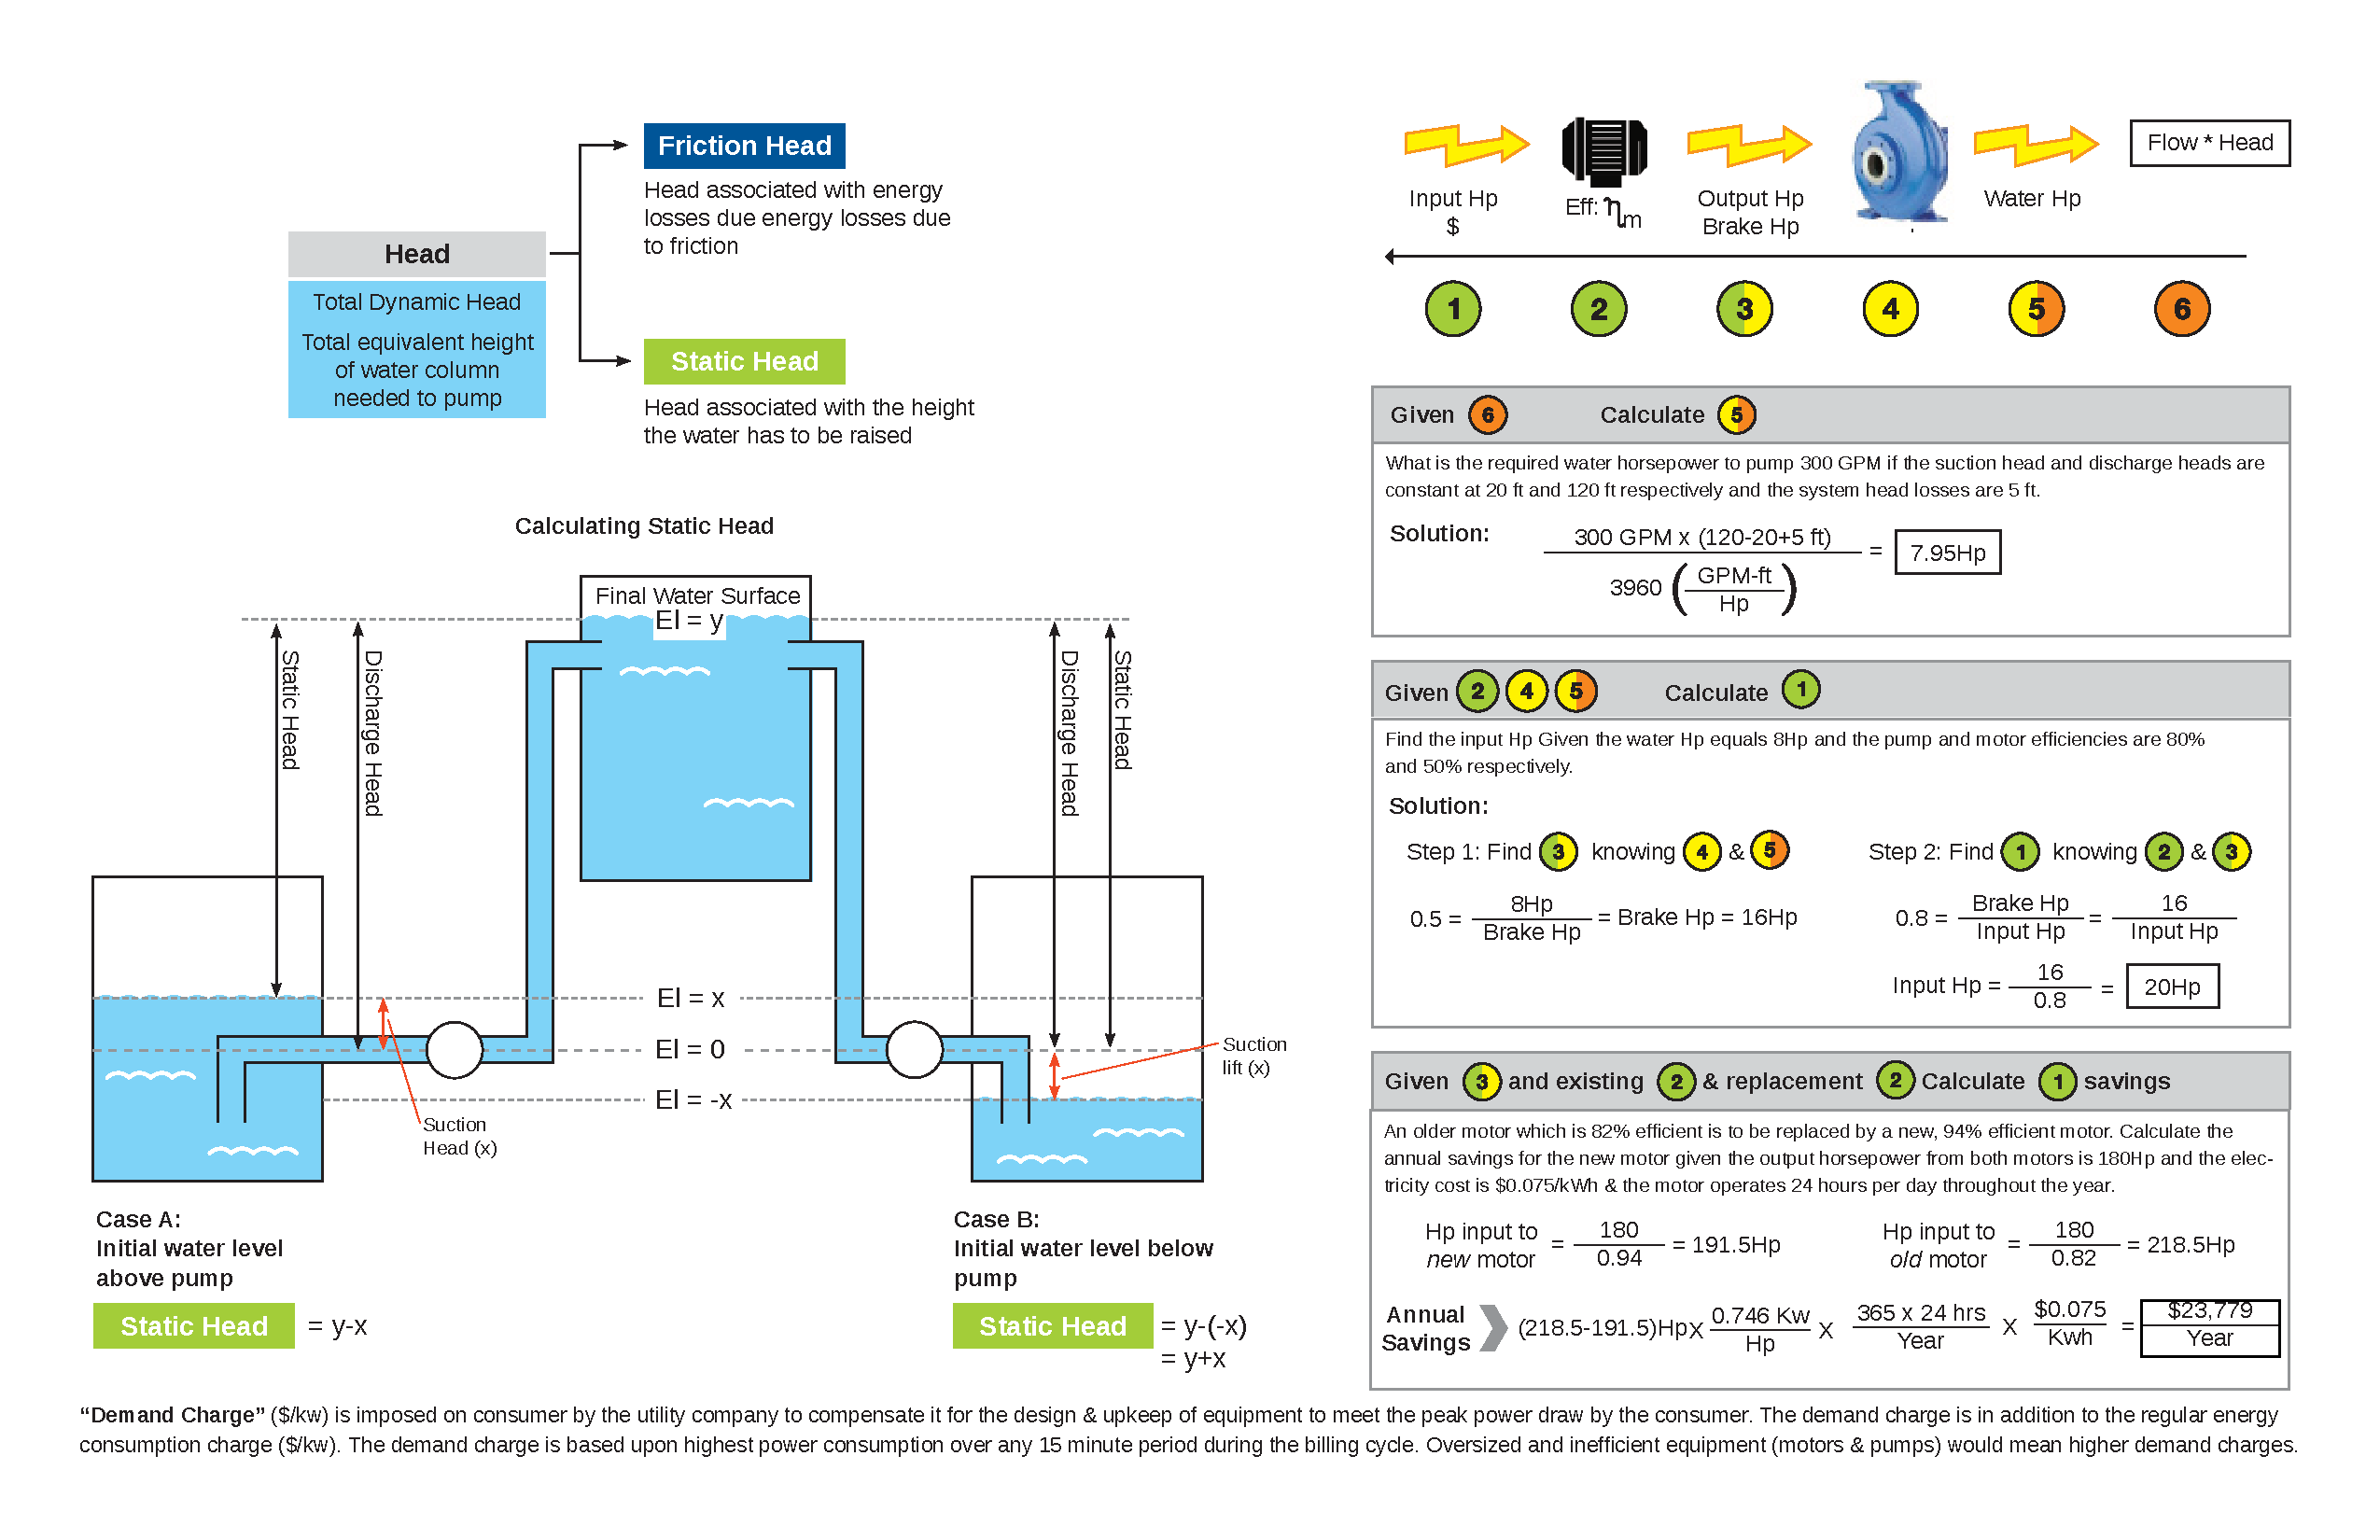
\includepdf[landscape=true]{PumpsandPumpingR1_02.pdf}
% \end{landscape}
\newpage

\section{Practice Problems}\index{Practice Problems}

\begin{enumerate}[1.]
\item 1 MGD is pumped against a 14’ head.  What is the water Hp?  The pump mechanical efficiency is 85\%.  What is the brake horsepower?\\
\vspace{0.4cm}
water Hp = flow * head\\
\vspace{0.4cm}
$\dfrac{1,000,000 \enspace gal}{day}*\dfrac{day}{1440 \enspace min}*14 \enspace ft*\dfrac{Hp}{3,960 \enspace GPM-ft}=\boxed{Water \enspace Hp = 2.46 \enspace Hp}$\\
\vspace{0.4cm}
pump Hp = brake Hp * pump efficiency\\
\vspace{0.4cm}
$Brake \enspace Hp = \dfrac{2.46}{0.85}=\boxed{Brake \enspace Hp=2.89Hp}$\\

\vspace{0.4cm}

\item A 8 ft diameter cylindrical wetwell receives an average incoming flow if 135 gpm and is pumped down with a pump that delivers 450 gpm again a total dynamic head of 120 ft.  The pump is controlled using two floats; a stop float located at 2.5 ft and a start float located at 16 ft.  If the pump motor is rated at 88\% and the pump at 77\%, what is the monthly (30 days/month) for running this pump if power costs are \$0.11/Kwh?\\


\vspace{0.4cm}
When the pump is on, the volume of wetwell that will be pumped down with the 450 gpm pump and a 135 gpm flow to the wetwell:\\
\vspace{0.4cm}
$\dfrac{450 \enspace gal}{min}-\dfrac{135 \enspace gal}{min}=\dfrac{315 \enspace gal}{min}$\\
\vspace{0.4cm}
Minutes required to pump down the wetwell :\\
\vspace{0.4cm}
$0.785*8^2*(16-2.5)ft^3*\dfrac{7.48 \enspace gal}{ft^3}*\dfrac{min}{315 \enspace gal}=16.1 \enspace min$\\
\vspace{0.4cm}
Time to fill wetwell with pump off @135gal/min influent flow:
\\
\vspace{0.4cm}
$[0.785*8^2*(16-2.5)]ft^3*\dfrac{7.48 \enspace gal}{ft^3}*\dfrac{min}{135 \enspace gal}=37.6min$\\
\vspace{0.4cm}
\# of cycles per day:\\
\vspace{0.4cm}
$\dfrac{cycle}{(16.1+37.6) \enspace min}*\dfrac{1440 \enspace min}{day}=\dfrac{26.8 \enspace cycles}{day}$\\
\vspace{0.4cm}
\# of hrs pump operational:\\
\vspace{0.4cm}
$\dfrac{16.1 \enspace min}{cycle}*\dfrac{26.8 \enspace cycles}{day}*\dfrac{hrs}{60 \enspace min}=\dfrac{7.19 \enspace hours}{day}$\\
\vspace{0.4cm}
Monthly electrical cost:\\
\vspace{0.4cm}
$\dfrac{450 \enspace gpm*120 \enspace ft}{0.88*0.77}*\dfrac{Hp}{3,960 \enspace gpm-ft}*\dfrac{0.746 \enspace kW}{Hp}*\dfrac{7.19hrs}{day}*\dfrac{30 \enspace days}{month}*\dfrac{\$0.11}{kWh}=\boxed{\dfrac{\$356}{month}}$\\
\vspace{0.4cm}

\item A 6-year old pump motor is to be replaced at a net cost of \$15,800. The new motor, just like the old one, would run 65\% of the time. Both existing and replacement motors would operate at 125 output Hp. The existing motor efficiency is 86\% while the replacement motor would be guaranteed at 94\% efficiency. Electricity currently averages \$0.088 per kWh.\\
\vspace{0.4cm}
(a) Calculate the energy cost savings per year (to the nearest dollar) if the existing motor is replaced with the new motor (neglect any consideration of impact upon demand charges or interest on capital).\\
\vspace{0.4cm}
(b) What is payback period to the nearest tenth of a year.\\
\vspace{0.4cm}
Solution:\\
\vspace{0.4cm}
Calculate energy cost savings per year:\\
\vspace{0.4cm}
Input Hp for old motor:$\dfrac{125}{0.86}=145.35Hp$\\
\vspace{0.4cm}
Input Hp for old motor:$\dfrac{125}{0.94}=132.98Hp$\\
\vspace{0.4cm}
Energy cost savings:\\$(145.35-132.98)Hp*\dfrac{0.746 \enspace kW}{Hp}*\dfrac{(365*24*0.65)hrs}{yr}*\dfrac{\$0.088}{kWh}=\boxed{\dfrac{\$4,624}{yr}}$\\
\vspace{0.4cm}
Calculate payback:\\
\vspace{0.4cm}
$\$15,800*\dfrac{yr}{\$4,623.94}=\boxed{3.4yr}$


\end{enumerate}
